% !TEX root = set_recommendation.tex
\section{Experiments}
\label{sec:experiments}

We study the performance of \acrlong{rfs} on two datasets. The first data
consists of researcher reading behavior from the arXiv; the task is to recommend
documents to scientists. The second is crowdsourced food consumption data from a
diet tracking app, and the task is meal recommendation. On both benchmarks,
\gls{rfs} outperforms several baseline methods.

\paragraph{Reproducibility} An example implementation is in \Cref{sec:code} and anonymized code for running
the simulation study in \Cref{sec:simulation} is at
% \url{https://github.com/kdd-anonymous/rankfromsets} (data cannot be shared, as
anon-url (data cannot be shared, as releasing diet or arXiv data is associated
with several privacy concerns).
%Code
%for training \gls{rfs} is available in the supplementary material.
% TODO: post-publication
% publicly available at \url{https://github.com/altosaar/rankfromsets}.

\subsection{Baselines}
\label{subsec:experiments:baselines}
We compare \gls{rfs} to a suite of recommendation models that rank items using
their sets of attributes.

\paragraph{Word embedding model.} We fit a word embedding
model~\citep{mikolov2013distributed} on the training data using the
implementation of fastText from \citet{bojanowski2017enriching}. The
dimensionality of the embeddings is set to match models being compared to. We
use a context window in the model that is slightly different than in the
original implementation. For an item with attributes $x_m$, the context for
attribute $j\in x_m$ is the set of other attributes of the same item
${j' \in x_m: j'\neq j}$. After learning the attribute embeddings $\beta_j$
for $j \in V$, item embeddings are computed as the average of their attribute
embeddings. Users are represented as the average of the embeddings of the items
they consume. Recommendation is performed by cosine similarity of an item
embedding and a user embedding.

% This is an order-invariant model. The
% output of the model (the cosine similarity) is invariant to the ordering of the
% attributes of an item: the item embeddings are computed as the average of
% attribute embeddings, and summation is invariant to permutation.

\paragraph{Collaborative topic Poisson factorization.} This is a probabilistic
matrix factorization model of user consumption data. The recommendation model
follows a latent variable scheme,

\begin{enumerate}
\item {\bf Document model:}
\begin{enumerate}
\item Draw topics $\beta_{vk} \sim \Gam(a, b)$
\item Draw document topic intensities $\theta_{dk} \sim \Gam(c, d)$
\item Draw word count $w_{dv} \sim \Pois(\theta_d^T \beta_v)$.
\end{enumerate}

\item {\bf Recommendation model:}
\begin{enumerate}
\item Draw user preferences $\eta_{uk} \sim \Gam(e, f)$
\item Draw document topic offsets $\epsilon_{dk} \sim \Gam(g, h)$
\item Draw $r_{ud} \sim \Pois(\eta_u^T (\theta_d + \epsilon_d))$.
\end{enumerate}
\end{enumerate}

\citet{gopalan2014content-based} develop a
variational inference algorithm for posterior inference in this model; we use
their implementation.

\paragraph{Collaborative topic Poisson factorization is a permutation-invariant
  recommendation model} To show that collaborative topic Poisson
factorization~\citep{gopalan2014content-based} is permutation-invariant,
consider the Poisson likelihood function over words $w_{dv}$. Conditional on the
latent item representation $\theta_d$ and latent word representation $\beta_v$,
every word in the document $w_{dv}$ is independent; the joint probability of
words in a document factorizes:
\begin{align}
  p(w_{d} \mid \theta_d, \beta_v) &= \prod_{w_{dv} \in w_d} p(w_{dv} \mid \theta_d, \beta_v).
\end{align}
In this model, predictions are made using expectations under the posterior. The
posterior is proportional to the the log joint of the model, and the attributes
of items (words in documents) enter into the model only via the above product.
The product of the probability of words in a document is invariant to a
reordering of the words in the document. Therefore, collaborative topic Poisson
factorization is permutation-invariant.

\paragraph{Permutation-marginalized recurrent neural network.} The Bernoulli
distribution used in \Cref{eqn:rankfromsets} can be parameterized using a
recurrent neural network. We treat attributes as a sequence and marginalize over
all permutations of orderings,
\begin{equation}
\label{eq:lstm}
\begin{aligned}
  p&(\yum = 1 \mid x_m) = \\
  &\frac{1}{\lvert \pi(x_m) \rvert}\sum_{\pi \in \pi(x_m)}\sigma
    \left(\phi(\theta_u,\{\beta_{\pi(1)}, \ldots, \beta_{\pi(J)}\})\right) \, .
\end{aligned}
\end{equation}
Here $\beta_j$ are attribute embeddings, $\pi(x_m)$ denotes the set of all
permutations of the set $x_m$, and $\phi$ is output of an LSTM recurrent neural
network~\citep{hochreiter1997long} projected to one dimension using a linear
layer. This model is permutation-invariant as there is an explicit sum over all
permutations.

\subsection{Recommending research papers}
\label{sec:experiments_arxiv}
We benchmark \gls{rfs} on data of scientists reading research
papers on the arXiv, where the goal is to recommend papers to scientists. The
arXiv usage data represents one year of usage (2012) and consists of $65$k
users, $637$k preprints, and $7.6$M clicks.

\paragraph{Evaluation.} We follow~\citet{gopalan2014content-based} and use the
same test and validation splits, and the same set of held-out $10$k users. To
match \citet{gopalan2014content-based}, we compute precision in addition to recall. The held-out
validation and test splits each consist of $20\%$ of the ratings and $1\%$ of
the documents. In-matrix documents refer to documents that have clicks in the
training data, while out-matrix or cold-start documents have no previous clicks.

\paragraph{Hyperparameters for \gls{rfs}.} We test the stochastic gradient
descent algorithm with and without momentum
\citep{sutskever2013on-the-importance}. We use a linear learning rate decay that
decays to zero in the maximum number of iterations, $200$k. We perform a grid
search over learning rates of ${1, 5, 10, 15, 25}$ and momenta of
${0.5, 0.9, 0.95, 0.99}$. The minibatch size is set to $\{2^{16}\}$. We use a
single negative sample per datapoint, sampled uniformly over the entire dataset
(corpus sampling is defined in \Cref{subsec:rankfromsets:negative-sampling}). To
match the hyperparameters in \citet{gopalan2014content-based}, we set the
dimensionality of embeddings to $100$. Evaluation is performed every $20$k
iterations.
% We did
% not test the residual or deep architectures on this dataset, as the large batch
% sizes did not fit in memory on the graphics processing unit we used.

\paragraph{Hyperparameters for the permutation-marginalized recurrent neural
  network.} The embedding and hidden state sizes are fixed to $100$. Evaluation
is performed every $20$k iterations. We grid search over learning rates of
${10^{-1}, 10^{-2}, 10^{-3}}$ with the Adam optimizer \cite{kingma2015adam:}. If
validation performance does not improve, we reload the best parameters and
optimizer states, and decay the learning rate by~$0.9$. We subsample single
permutations during training and testing.


\paragraph{Results.} \Cref{fig:arxiv-performance} shows that \gls{rfs} with the
inner product parameterization outperforms collaborative topic Poisson
factorization in terms of in-matrix recall by over $90\%$. It also improves over
\gls{ctpf} in terms of out-matrix recall, out-matrix precision, and in-matrix
precision (for the latter, only when the number of recommendations is greater
than $30$). The word embedding model performs about as well as \gls{ctpf} in
terms of recall, but performs worse in terms of precision. The
permutation-marginalized recurrent neural network model performance was an order
of magnitude worse than the other methods; we report its performance in
\Cref{tab:lstm-arxiv}.
%; we report these results in\Cref{sec:appendix-lstm}.
% Too subjective and seems like conjecture: let the reader decide this
% This provides empirical support for using a
% classifier as a recommender as \Cref{prop:maximizing-recall} suggests, and shows that
% \gls{rfs} encompasses the performance gains of existing matrix
% factorization and deep learning models.

Qualitatively, \gls{rfs} reveals patterns in usage of the arXiv.
\Cref{fig:arxiv_tsne} is a dimensionality-reduced plot of the user embeddings
that reveals connections between fields of study. Scientists who focus on high
energy physics, \texttt{hep}, neighbor specialists in differential geometry,
\texttt{math.DG}; these areas share techniques. Machine learning researchers,
\texttt{stat.ML} readers, neighbor statisticians or \texttt{math.ST} readers,
highlighting the close connection between these fields. Plots for document
embeddings show similar patterns. This illustrates how \gls{rfs}
captures rich patterns of interaction between users and items, while benefitting
from information in the item attributes.

\subsection{Recommending meals}
\label{sec:experiments_meals}

We evaluate \gls{rfs} on data collected from the LoseIt! food tracking app. This
app enables users to track their food intake to eat healthy. We use a year's
worth of data from $55$k active users. This corresponds to $16$M meals, where
each meal is comprised of a subset of $3$M foods.

\paragraph{Preprocessing.} Each meal is a subset of $3$M foods. We filter the
vocabulary by keeping words that occur at least 20~times in the food names,
resulting in $9963$~words. A meal is represented as the union of the sets of
words occurring in the food names.

\paragraph{Evaluation.} We hold out 1\% of the items (meals) for validation and
hold out 1\% of the items for evaluating test performance. We use the sampled
recall metric in \Cref{eq:sampled-recall} with $K=10$. 

\begin{figure}[!tb]
  \centering
  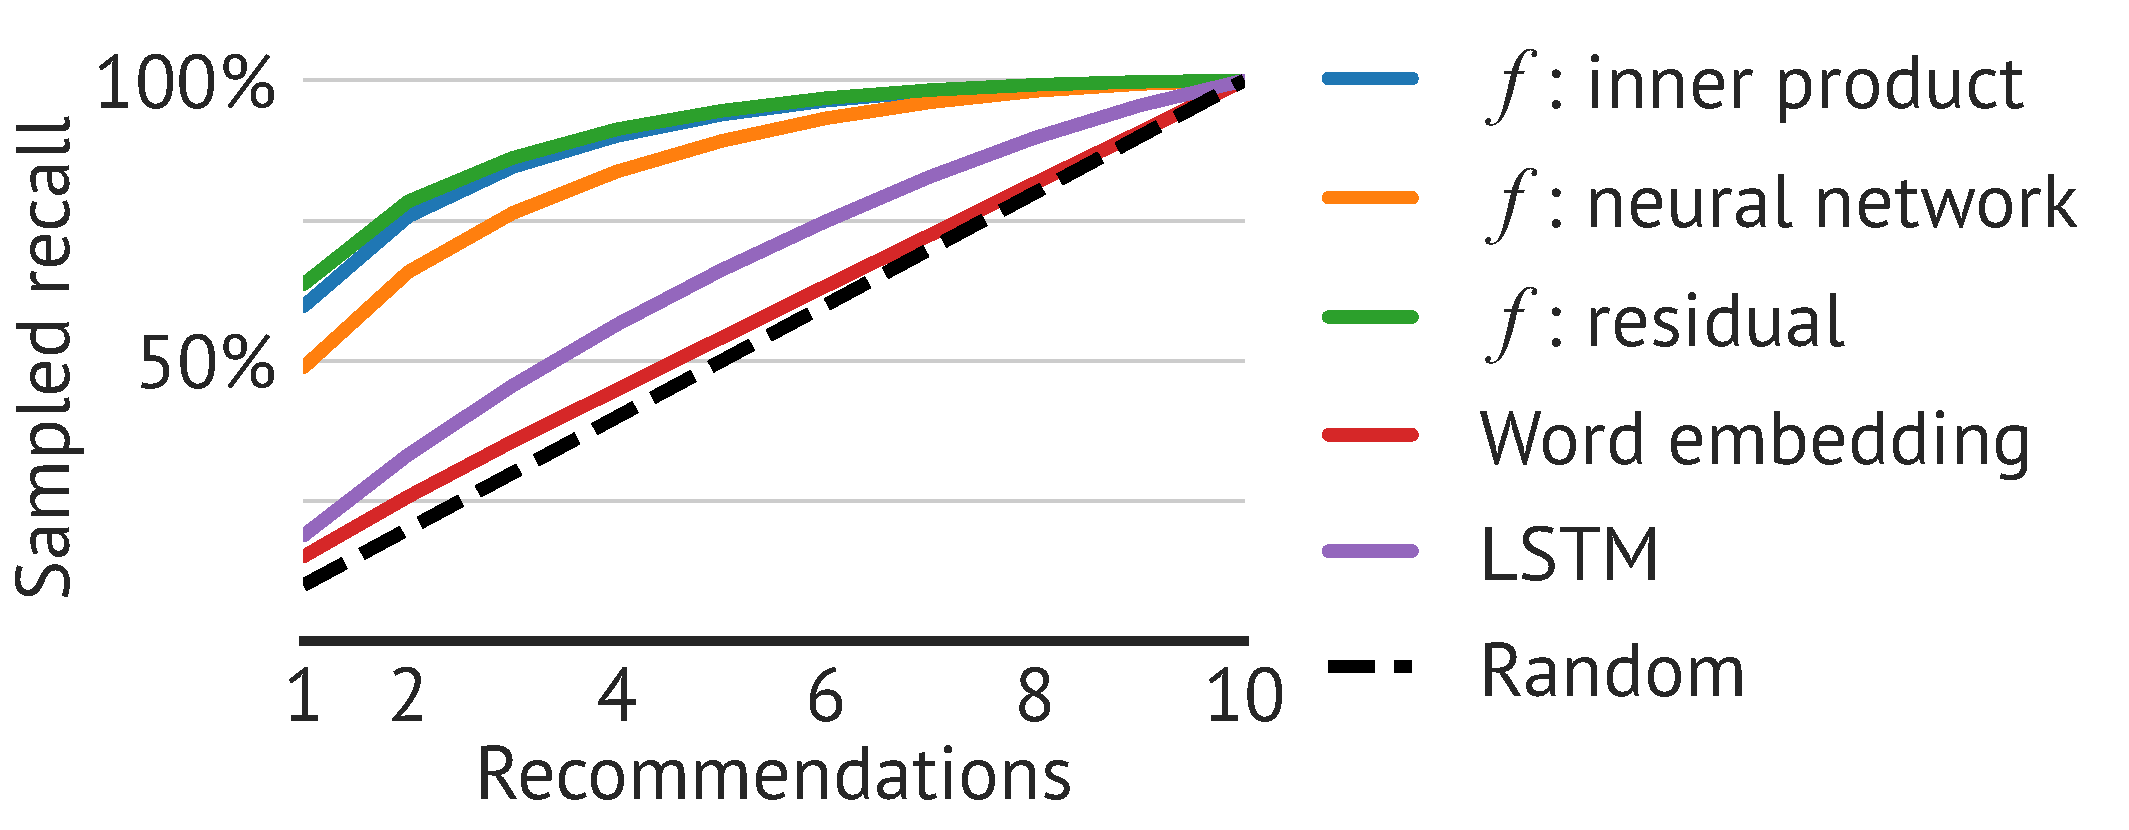
\includegraphics[width=0.95\linewidth]{fig/meal-recall}
  \caption{\acrlong{rfs} outperforms models based on word embeddings
    permutation-marginalized recurrent neural networks (denoted by LSTM) on meal
    recommendation. The recommendation models are trained on data from a food
    tracking app as described in \Cref{sec:experiments_meals} and are evaluated
    using the sampled recall metric, \Cref{eq:sampled-recall}. The inner
    product, neural network, and residual regression functions for \acrlong{rfs}
    are in \Cref{eqn:rankfromsets,eqn:neural-network,eqn:residual}.}
  \label{fig:meal-recall}
\end{figure}

%%% Local Variables:
%%% mode: latex
%%% TeX-master: "../set_recommendation"
%%% End:

\begin{table*}[!hbpt]
\centering
\begin{tabular}{p{80mm}|p{80mm}}
  \toprule
  Query meal & Nearest meal by cosine similarity \\
  \midrule
  Two scoops of Raisin Bran cereal, organic Moroccan green tea, almond milk,
  light honey, tap water, large banana, large strawberries
       &
         Vita Bee bread, salted butter, fresh medium tomatoes, large fried whole
         egg, small banana\\\hline
  Iceberg lettuce, cantaloupe cubes, diced honeydew melon, cherry tomatoes, olives, dry-cooked unsalted
  hulled sunflower seed kernels, chopped hard-boiled
  egg, cucumbers, dried cranberries, fat-free ranch dressing
       &
         Green leaf lettuce, chopped sweet red bell peppers, crumbled feta cheese,
         large hard-boiled egg,
         chopped cucumber, oil-roasted salted sunflower seeds, sliced radishes, sliced strawberries, pitted Calamata olives, fat-free
         balsamic vinegar\\\hline
  Boston roast pork, mackerel, artichoke hearts, spinach, pimiento-stuffed
  Manzanilla olives, carrots, mushrooms, peppercorn ranch dressing
       &
         Broiled top
         round steak, tomatoes, cucumber, baby yellow squash, zucchini, black olives,
         extra
         virgin
         olive oil\\\hline
  Meatloaf with tomato sauce, chopped sweet red bell peppers, extra virgin olive oil, cooked asparagus spears, sweet potatoes, orange, cantaloupe cubes
       &
         Chicken breast, breadcrumbs, fresh tomatoes, shredded green leaf
         lettuce, extra virgin olive oil, spinach, chopped yellow onion, sweet
         large yellow bell peppers, whole mushrooms, chili peppers, vinaigrette
  \\\hline
  Ciabatta bun, cooked skinless chicken breast, fresh baby spinach, shredded iceberg lettuce,
  shredded mozzarella cheese, ketchup, frozen yogurt bar
             &
               Small whole wheat submarine roll, broiled round roast
               beef, roasted light turkey meat without skin, fresh medium
               tomatoes, honey smoked ham, shredded iceberg lettuce, sliced mozzarella cheese\\
         \bottomrule
\end{tabular}
\caption{\acrlong{rfs}, trained on food consumption data, provides diverse
  recommendations. We fit the model to data from a food tracking app as
  described in \Cref{sec:experiments_meals}; items are meals and attributes are
  the ingredients in the meal. We represent meals as the mean of their attribute
  embeddings, and use cosine similarity to compute the nearest neighbors of
  meals. This reveals that \acrlong{rfs} uncovers latent patterns of consumption
  in the attribute embeddings that can be leveraged to improve recommendations.
  For example, the second-last query meal is a mix of meat, vegetables, and
  fruit, and the nearest neighbor meal is a different meat and a side of salad.
  The last query meal is a sandwich, and its nearest neighbor is also a
  sandwich, but with different ingredients.}
\label{tab:nearest_meals}
\end{table*}

%%% Local Variables:
%%% mode: latex
%%% TeX-master: "../set_recommendation"
%%% End:


\paragraph{Hyperparameters for \gls{rfs}.} The embedding size is set to $128$.
For the neural network and residual models in
\Cref{eqn:neural-network,eqn:residual} the number of hidden layers is two, and
the number of hidden units is set to $256$. The item embeddings $g(x_m)$, and
item intercepts $h(x_m)$, are computed as the mean of learned food embeddings or
intercepts, respectively. We use the RMSProp optimizer in
\citet{graves2013generating} and grid search over learning rates in
$\{10^{-2}, 10^{-3}, 10^{-4}, 10^{-5}\}$. We use a batch size of $64$ and a
single negative sample for every datapoint in a minibatch (batch sampling is
defined in \Cref{subsec:rankfromsets:negative-sampling}). Evaluation is
performed every $50$k iterations.

% For the neural
% network and residual models in \Cref{eq:neural-network,eq:residual}
% respectively, we use a two-hidden-layer neural network with rectifier
% nonlinearities and $256$~hidden units per layer. 

\paragraph{Hyperparameters for the permutation-marginalized recurrent neural
  network.} We grid search over batch sizes of $\{32, 64, 128\}$. For every item
in a minibatch, we sample a single permutation of attributes to approximate the
sum in \Cref{eq:lstm}. We use a single negative sample per datapoint, and set
the embedding and hidden state sizes to $128$. We use the Adam
optimizer~\citep{kingma2015adam:} and grid search over learning rates of
$\{10^{-2}, 10^{-3}, 10^{-4}\}$. Evaluation is performed every $1$k iterations.
If the validation performance does not improve, we reload the best parameters
and optimizer states, and decay the learning rate by $0.9$.

\paragraph{Results.} \Cref{fig:meal-recall} plots the sampled recall. This shows
that \gls{rfs} outperforms the permutation-marginalized recurrent neural network
and the word embedding model. The code released by the authors of the
collaborative topic Poisson factorization model
in~\cite{gopalan2014content-based} did not scale to this size of data.

% In \gls{rfs}, the
% residual parameterization is the most flexible and marginally outperforms the
% other models. 
% , despite several attempts on systems with sufficient
% computational resources.
Qualitatively, \gls{rfs} learns an interpretable representation of
items, as shown by nearest neighbors of meals in \Cref{tab:nearest_meals}. In
this table, we display breakfast, lunch, and dinner meals, alongside their
nearest neighbors. We find that the nearest neighbors are also breakfast, lunch,
and dinner meals respectively, showing that the attribute embeddings learned by
the model can be used to explore qualitative patterns in the learned latent
space.
%  To
% confirm that the learned latent embedding space was interpretable,
% dimensionality-reduced plots of user embeddings were labeled according to user
% demographics such as age. This showed that similar users (in terms of covariates
% and eating habits) are placed in similar parts of the latent space.%  A similar
% analysis of meals was conducted, but no pre-existing labels exist. Manual
% inspection revealed that similar meals are learned to be put in similar latent
% regions (mirroring \Cref{tab:nearest_meals}).

%%% Local Variables:
%%% mode: latex
%%% TeX-master: "set_recommendation"
%%% End: